\appendix

\section{Signal Correlation}
\label{app:correlation}

\begin{figure}[H]
    \centering
    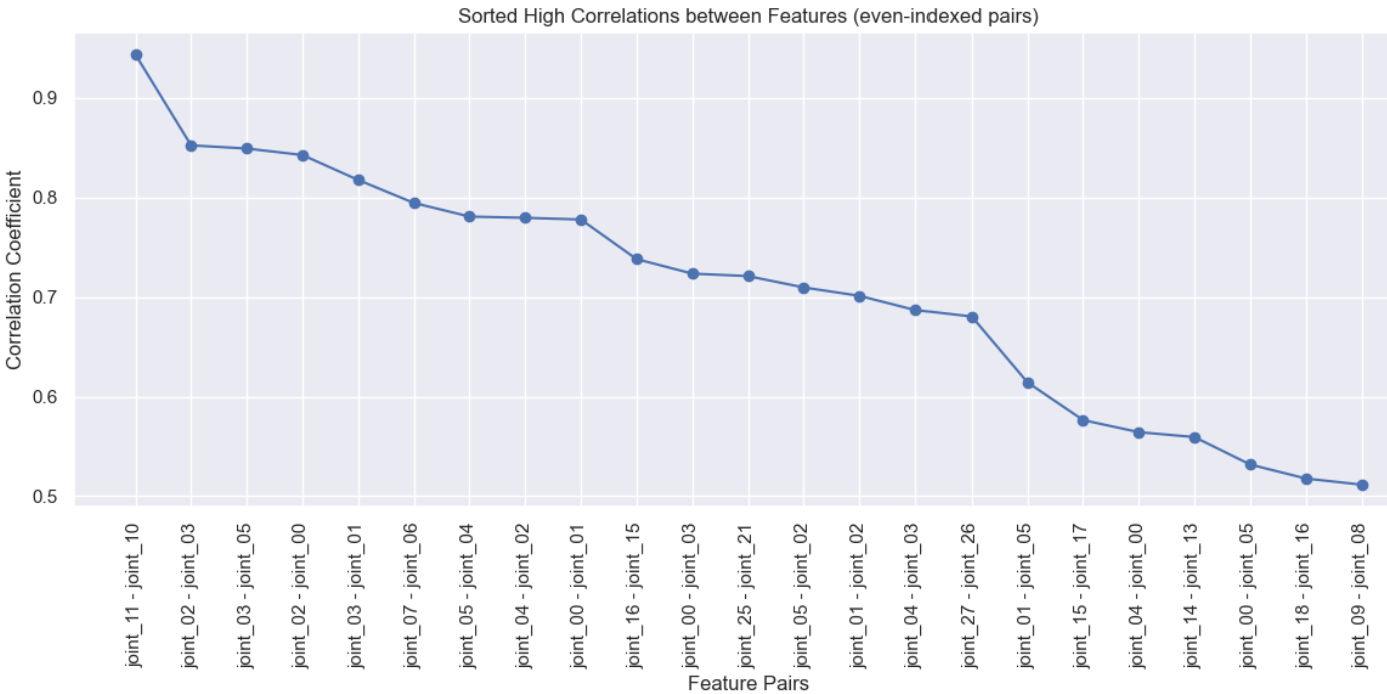
\includegraphics[width=\linewidth]{Deliverables/Report1/img/correlation_10_11.png}
    \caption{High correlated features plot}
    \label{fig:correlation_10_11}
    \vspace{-20pt}
\end{figure}
\begin{figure}[H]
    \centering
    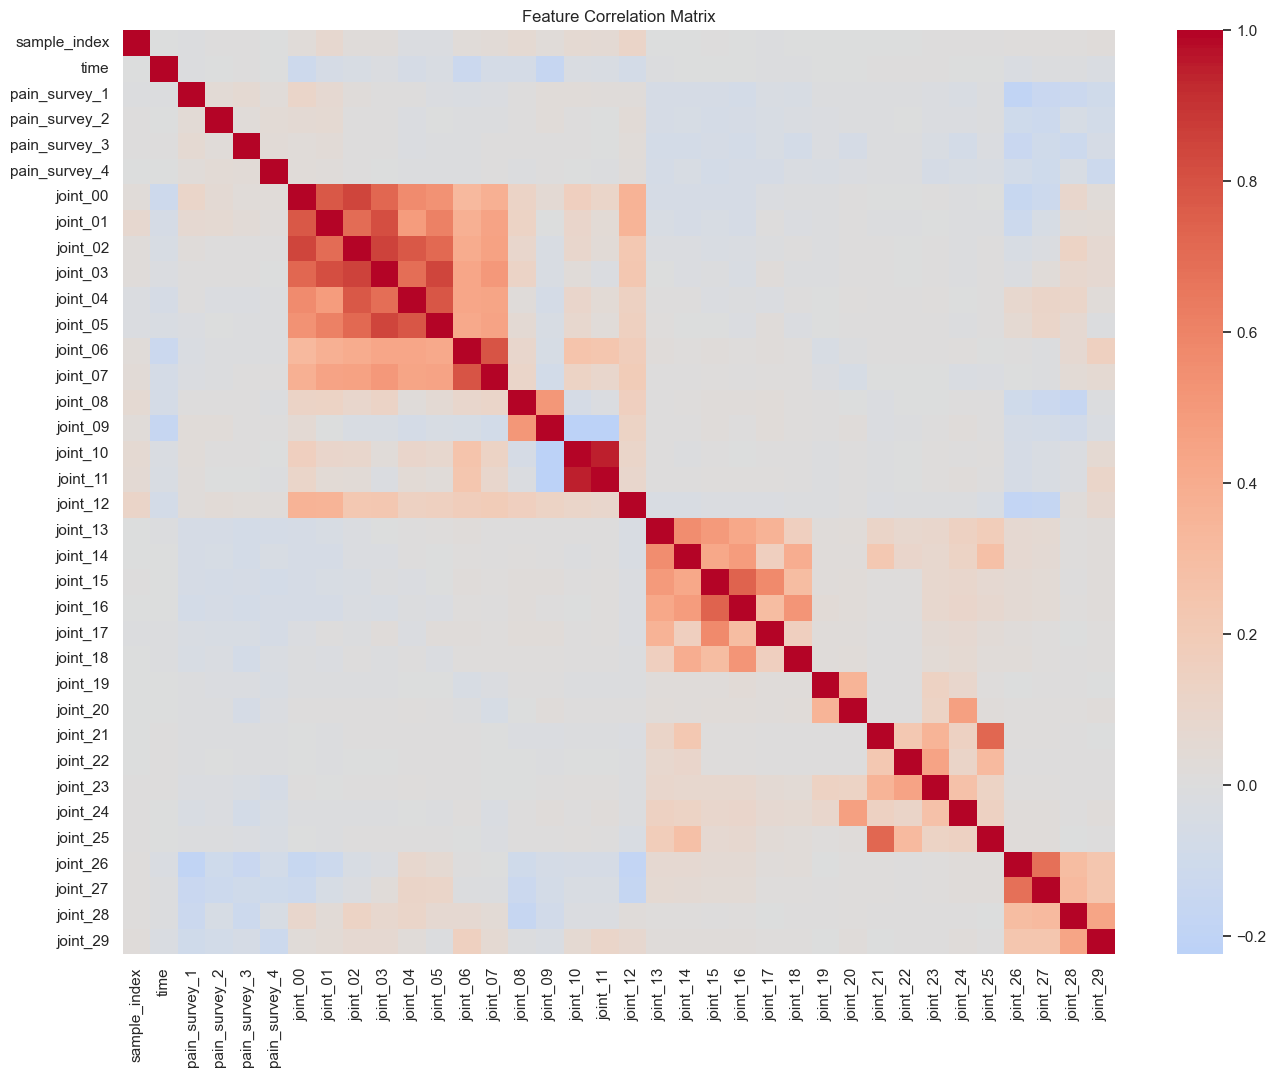
\includegraphics[width=\linewidth]{Deliverables/Report1/img/correlation_matrix.png}
    \caption{High correlated features matrix}
    \label{fig:correlation_10_11}
    \vspace{-20pt}
\end{figure}


\section{PCA}
\label{app:pca}

PCA is applied independently to each trajectory 
$x_{i,f} = (x_{i,f}(1),\ldots,x_{i,f}(T))^\top \in \mathbb{R}^T$. 
PCA yields $x_{i,f} \approx U_f z_{i,f}$, where $U_f$ contains the leading 
eigenvectors and $z_{i,f}$ the corresponding POD coefficients. The number 
of retained components is the minimum $k$ such that
\[
\sum_{j=1}^{k} \lambda_{f,j} \ge 0.95 \sum_{j=1}^{T} \lambda_{f,j},
\]
and the resulting POD coefficients are appended to the global feature vector.
\begin{figure}[H]
    \centering
    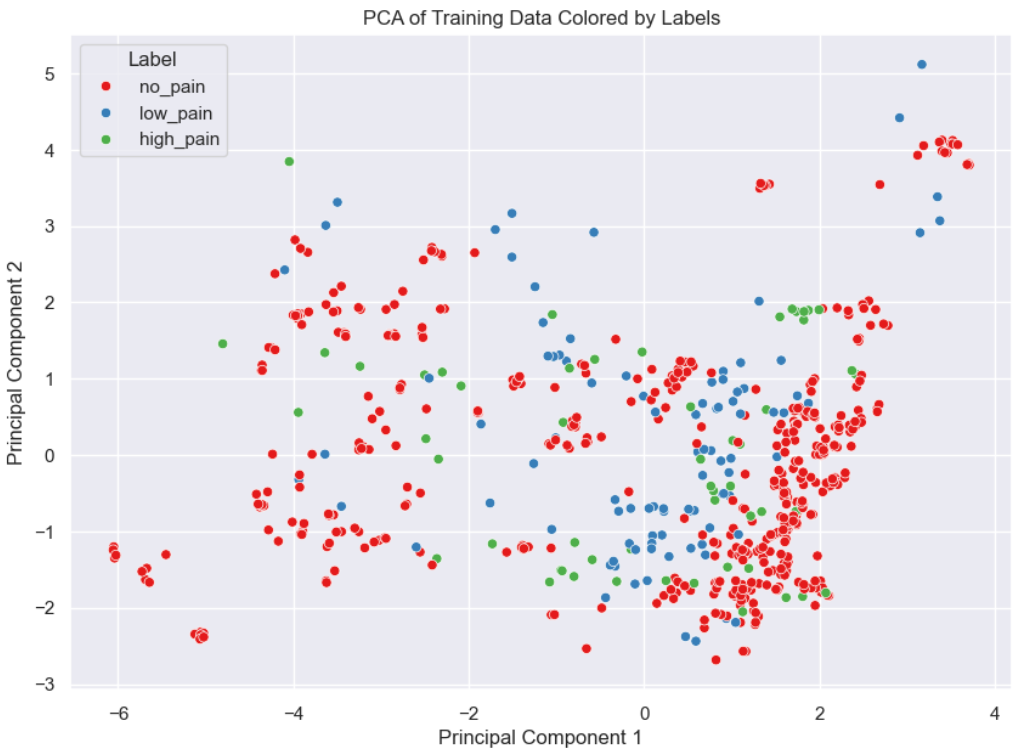
\includegraphics[width=\linewidth]{Deliverables/Report1/img/pca.png}
    \caption{PCA on training data}
    \label{fig:correlation_10_11}
    \vspace{-20pt}
\end{figure}

\section{Experimental plots}
\label{app:plots}
\begin{figure}[H]
    \centering
    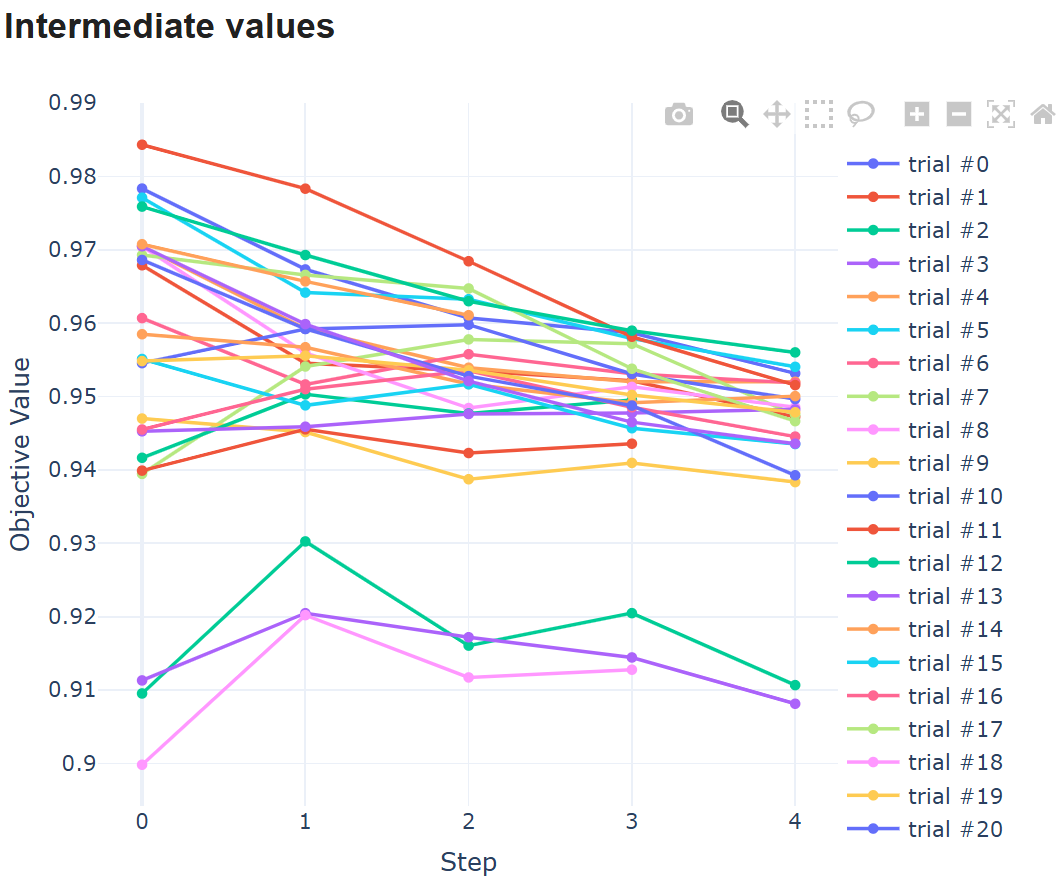
\includegraphics[width=\linewidth]{Deliverables/Report1/img/optuna4.png}
    \caption{Fold F1Score}
    \label{fig:correlation_10_11}
    \vspace{-20pt}
\end{figure}
\begin{figure}[H]
    \centering
    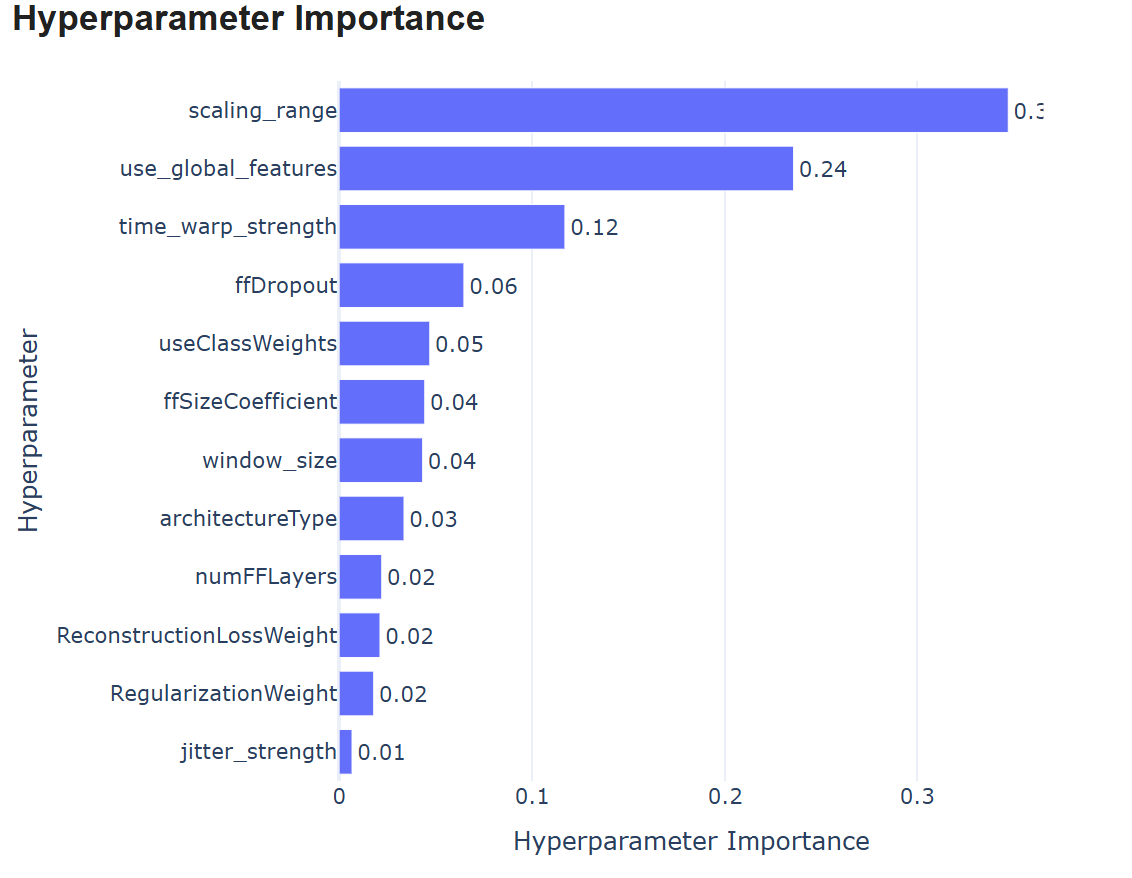
\includegraphics[width=\linewidth]{Deliverables/Report1/img/optuna3.png}
    \caption{Hyperparameter importance}
    \label{fig:correlation_10_11}
    \vspace{-20pt}
\end{figure}
\begin{figure}[H]
    \centering
    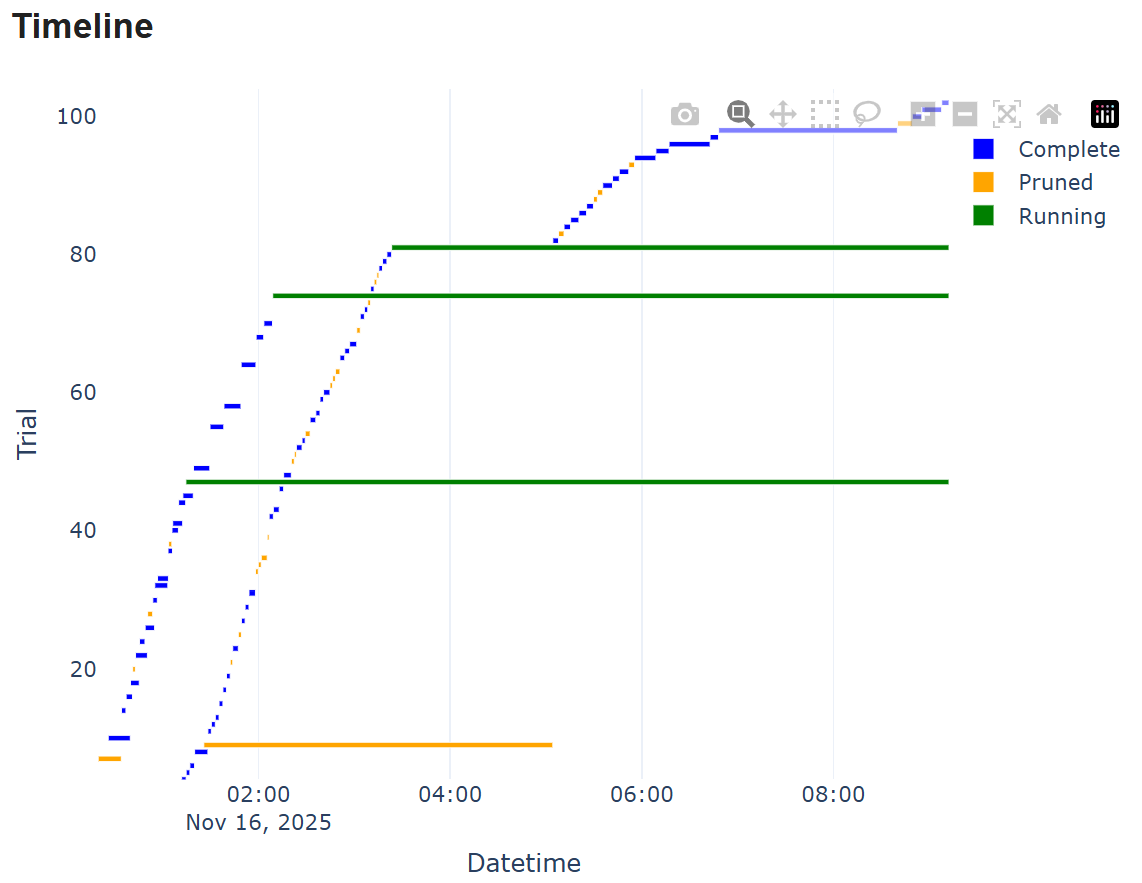
\includegraphics[width=\linewidth]{Deliverables/Report1/img/optuna5.png}
    \caption{Timeline}
    \label{fig:correlation_10_11}
\end{figure}
\section{Results}
\begin{figure}[H]
    \centering
    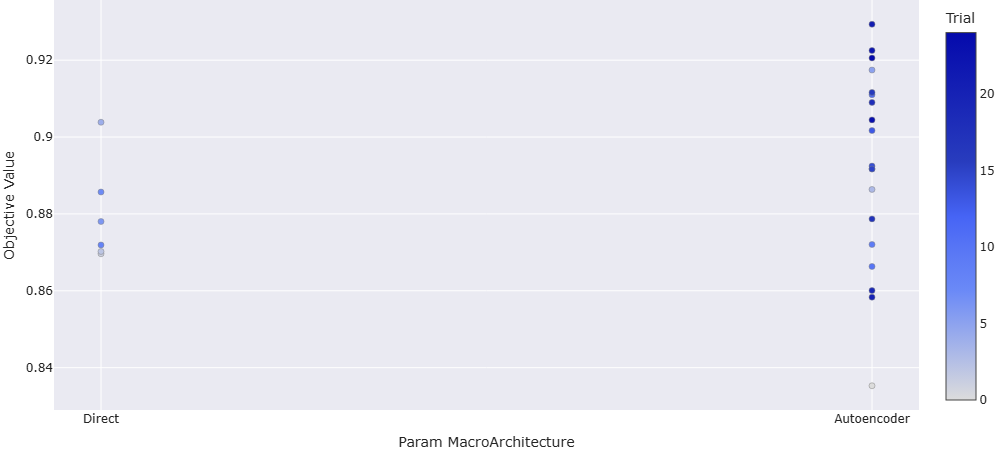
\includegraphics[width=\linewidth]{Deliverables/Report1/img/AutoencodervsDirect.png}
    \caption{Autoencoder vs Direct performances}
    \label{fig:Optuna}
\end{figure}